\documentclass[english]{tktltiki}
\usepackage[pdftex]{graphicx}
\usepackage{subfigure}
\usepackage{enumerate}
\usepackage[table,xcdraw]{xcolor}
\usepackage{url}
\usepackage{mathtools}  
\usepackage{multirow}
\mathtoolsset{showonlyrefs}  
\begin{document}
\onehalfspacing

\title{Location Awareness - Home Exam}
\author{P�ter Ivanics}
\date{\today}

\maketitle

\numberofpagesinformation{\numberofpages\ pages + \numberofappendixpages\ appendices}
\keywords{}

\mytableofcontents

\section{Concepts}
	\begin{enumerate}[a)]
		\item Let us donate the length of the semi-major axis with $a = 6378137$ and the inverse flattening $1/f \approx 298.26$. Calculating the actual flattening we get $f = \frac{1}{298.26} \approx 3.35 * 10^{-3}$.  Then we use the equation of flattening to calculate $b$ as follows: 
		\begin{eqnarray*}
			f = \frac{a - b}{a} \\ \\
			3.35 * 10^{-3} = \frac{6378137 - b}{6378137} \\ \\
			3.35 * 10^{-3} * 6378137 = 6378137 - b \\ \\ 
			- 3.35 * 10^{-3} * 6378137 + 6378137 = b \\ \\ 
			b \approx 6356753
		\end{eqnarray*}
		
	\item To obtain the answer we shall calculate the Helsinki-Santiago and the Helsinki-Auckland distance. We use the Haversine formula \footnote{\url{https://en.wikipedia.org/wiki/Haversine_formula}} 
	\begin{gather}
		Dist([\phi_1, \lambda_1], [\phi_2, \lambda_2]) = 2 r \arcsin \sqrt{\sin^2 (\frac{\phi_2 - \phi_1}{2}) + \cos (\phi_1) * \cos (\phi_2) * \sin^2 (\frac{\lambda_2 - \lambda_1}{2})}
	\end{gather}
	to calculate the distances as follows (in kilometers) using $r = 6371$ kilometers and coordinates retrieved from Google:
	\begin{eqnarray*}
		Dist(Hel, San) = Dist([60.1699� N, 24.9384� E], [33.4489� S, 70.6693� W]) = 13480 \\
		Dist(Hel, Auc) = Dist([60.1699� N, 24.9384� E], [36.8485� S, 174.7633� E]) = 16660
	\end{eqnarray*}
	
	If the flying range of the plane is $r = 15190$ kilometers, it can reach Santiago without refueling and still have fuel for approximately $15190 - 13480 = 1710$ kilometers. However, it cannot reach Auckland without refueling as it would run out of fuel around $|15190 - 16660| = 1470$ kilometers before reaching the destination. 
	
	\item The attached $k-anonimity.R$ file contains an implementation for retrieving the answer for item c) and d). The calculated Euclidean distances between the given points are displayed in the table below. The $4^{th}$ smallest distance in the table is $d = 0.08331873$ which means to ensure k-anonymity of $k=4$, this value should be used as threshold. 
	
	\begin{table}[ht]
		\centering
		\begin{tabular}{rrrrrrrrrrr}
 		 \hline
 		& 1 & 2 & 3 & 4 & 5 & 6 & 7 & 8 & 9 & 10 \\ 
  		\hline
		1 & 0.00 & 0.26 & 0.27 & 0.11 & 0.17 & 0.18 & 0.15 & 0.21 & 0.16 & 0.24 \\ 
		 2 & & 0.00 & 0.28 & 0.26 & 0.18 & 0.34 & 0.27 & 0.13 & 0.16 & 0.04 \\ 
		 3 & & & 0.00 & 0.23 & 0.14 & 0.21 & 0.14 & 0.16 & 0.22 & 0.27 \\ 
		 4 & & & & 0.00 & 0.12 & 0.23 & 0.17 & 0.20 & 0.10 & 0.22 \\ 
		 5 & & & & & 0.00 & 0.21 & 0.13 & 0.08 & 0.08 & 0.16 \\ 
		 6 & & & & & & 0.00 & 0.08 & 0.24 & 0.27 & 0.33 \\ 
 		 7 & & & & & & & 0.00 & 0.17 & 0.19 & 0.26 \\ 
 		 8 & & & & & & & & 0.00 & 0.13 & 0.12 \\ 
 		 9 & & & & & & & & & 0.00 & 0.13 \\ 
  		10 & & & & & & & & & & 0.00 \\ 
   		\hline
		\end{tabular}
	\end{table}
	
	\item Using the given parameter the program outputs the following: \textit{"Parameters: eps = 0.15, minPts = 4. The clustering contains 1 cluster(s) and 0 noise points"}. This means that all points are grouped under the same cluster and all of them have dense neighborhoods. 
	\end{enumerate}
\section{Position Estimation}
	\begin{enumerate}[a)]
		\item As displayed on Figure \ref{user_position} below, the two circles of 7 meters intersect around the towers at points (14.42,4.57) and (7.58,3.43). Accordingly, the user can be located at one of these points or in their error prone. 
		
	\begin{figure}[h] 
		\begin{center}
			\caption{The intersection points of the 7-meter radius circles around the towers (up) and the uncertainty regions (down) of Exercise 3. }
			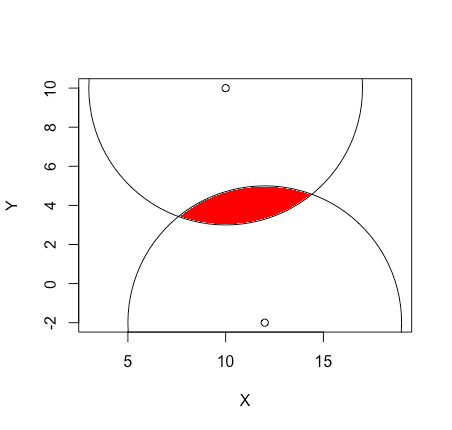
\includegraphics[width=0.8\textwidth]{images/user_position.png}
			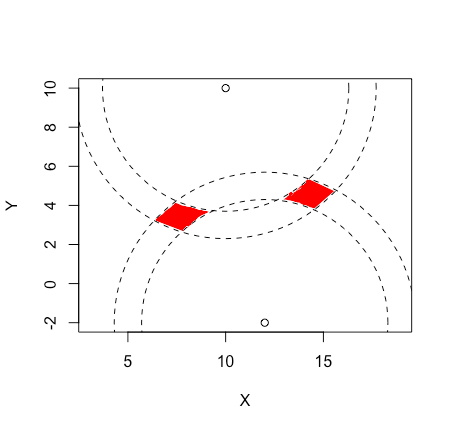
\includegraphics[width=0.8\textwidth]{images/user_position_with_error.png}
			\label{user_position}
		\end{center}
	\end{figure}
	
	\item Table \ref{intersection_points} lists the coordinates of the bounding points of the uncertainty regions with the given 10 \% error rate. 
	
	\begin{table}[]
		\centering
		\caption{The bounding coordinates of the uncertainty regions on Figure \ref{user_position} of Exercise 3. }
		\label{intersection_points}
		\begin{tabular}{lll}
			\hline
			\textbf{Error area} & \textbf{X} & \textbf{Y}    \\
			\hline 
			\multirow{4}{*}{Left} & 6.34  & 3.22 \\
					 							& 7.47  & 4.23 \\
			 									& 7.74  & 2.64 \\
			 									& 9.38  & 3.73 \\
			 \hline
			\multirow{4}{*}{Right} & 12.62 & 4.27 \\
												 & 14.26 & 5.36 \\
					 							& 14.53 & 3.77 \\
					 							& 15.66 & 4.78 \\
			\hline
		\end{tabular}
		\end{table}
		
		\item To calculate the maximum error rate, we calculate the size of the two error regions as follows. This way the Dilution of Precision (DoP) value is retrieved as the sum of the areas. To calculate the area of the polygons, the 
		$A = |\frac{(x_1 y_2 - y_1 x_2) + (x_2 y_3 - y_2 x_3) + ... + (x_n y_1 - y_n x_1)}{2}|$ 
		formula is used.
		
		\begin{gather}
			A_1 = |\frac{6.34 * 4.23 - 3.22 * 7.47 + ... 
				% 7.47 * 2.64 - 4.23 * 7.74 + 7.74 * 3.73 - 2.64 * 9.38 
				+ 9.38 * 3.22 - 3.73 * 6.34}{2}| 
			= \frac{0.4078}{2} = 0.2039 \\ 
			\\
			A_2 = |\frac{12.62 * 5.36 - 4.27 * 14.26 + ... 
			% 14.26 * 3.77 - 5.36 * 14.53 + 14.53 * 4.78 - 3.77 * 15.66 
			+ 15.66 * 4.27 - 4.78 * 12.62}{2}| = |\frac{-0.4078}{2}| = 0.2039 \\
			\\
			A = A_1 + A_2 = 2 * 0.2039 = 0.4078
		\end{gather}
		
	\end{enumerate}
\section{Spatial Analysis}
	The attached $spatial-analysis.R$ file was developed to carry out the solution for this task. 
	
	\begin{enumerate}[a)]
		\item The $preprocessData()$ function is tailored to perform noise-reduction of the data. The parameters are configured by default as follows: 
		\begin{itemize}
			\item minimumSatellites = 3,
			\item maximumHDOP = 6,
			\item rangeTreshold = 50 [meters]
		\end{itemize}				
		
		The attached $buenosaires-KML-original.kml$ contains the original, while the $buenosaires-KML-pruned.kml$ contains the reduced points according to the rules above. There were 712 points which got reduced to 334 points once the preprocessing was performed using the default parameters above. Figure \ref{buenosaires} displays the original (top) and the pruned (bottom) points on the map. We can see that some of the points, for example the rightmost ones in the ocean could be still removed.
		
		\begin{figure}[h] 
			\begin{center}
				\caption{The original (top, in total 712) and the pruned points (bottom, in total 334) on the Buenos Aires dataset visualized by KML. } 
				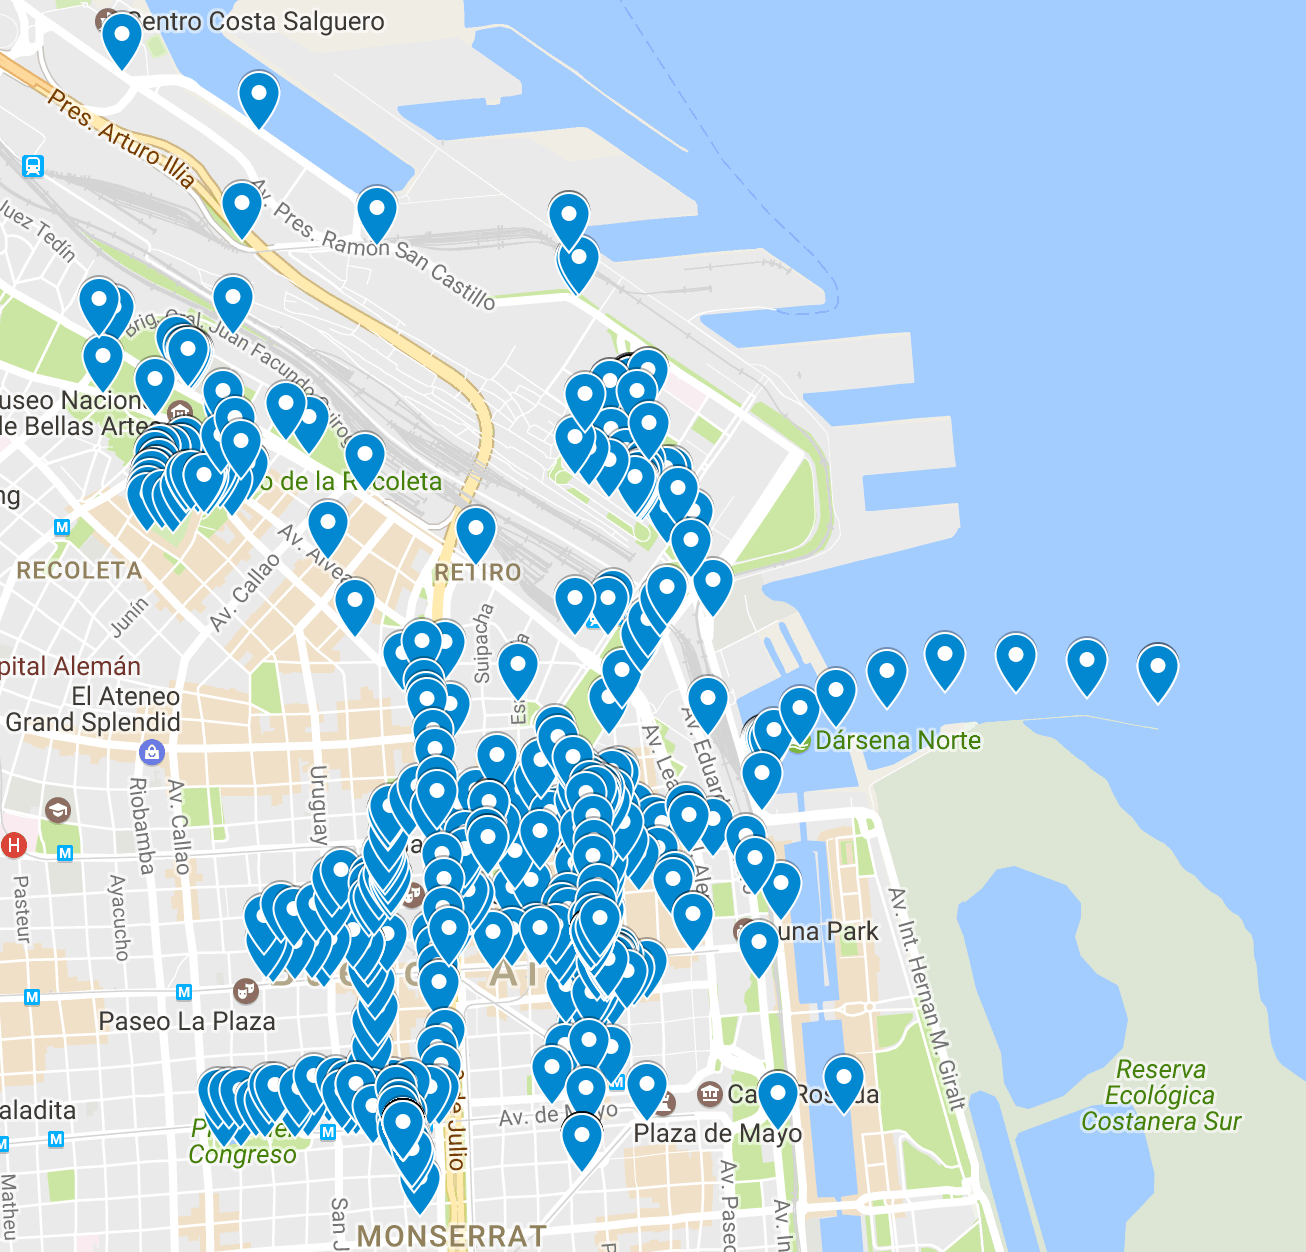
\includegraphics[width=0.8\textwidth]{images/buenosaires-original-kml.png} 
				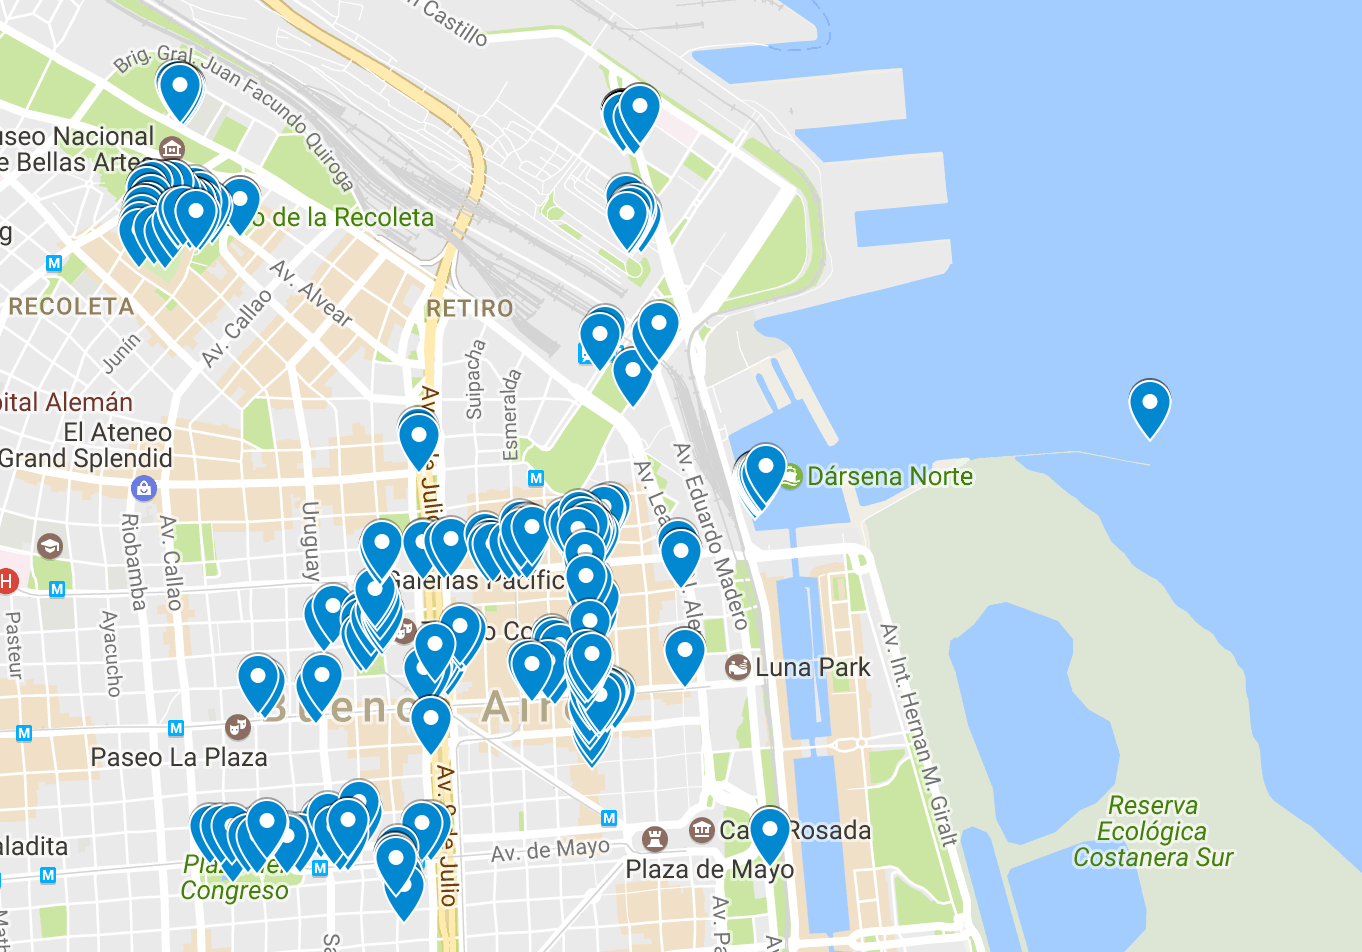
\includegraphics[width=0.8\textwidth]{images/buenosaires-pruned-kml.png}
				\label{buenosaires}
			\end{center}
		\end{figure}
	
		\item To perform the place identification, I have chosen the K-means algorithm. The $kmeans()$ function in the attached file performs the k cluster assignments. A simple Eucledian distance is used as distance measure. After trying out various values for k, I could identify 4 places in the dataset. Figure \ref{buenosaires-kmeans} displays the clusters and their centers (with '+' marks) with different colors. We can see that the assignment of the black and green points is probably not perfect.
		
		\begin{figure}[h] 
			\begin{center}
				\caption{One result of the K-means algorithm using $k=4$ on the pruned points ($buenosaires-KML-pruned.kml$) of the Buenos Aires dataset.} 
				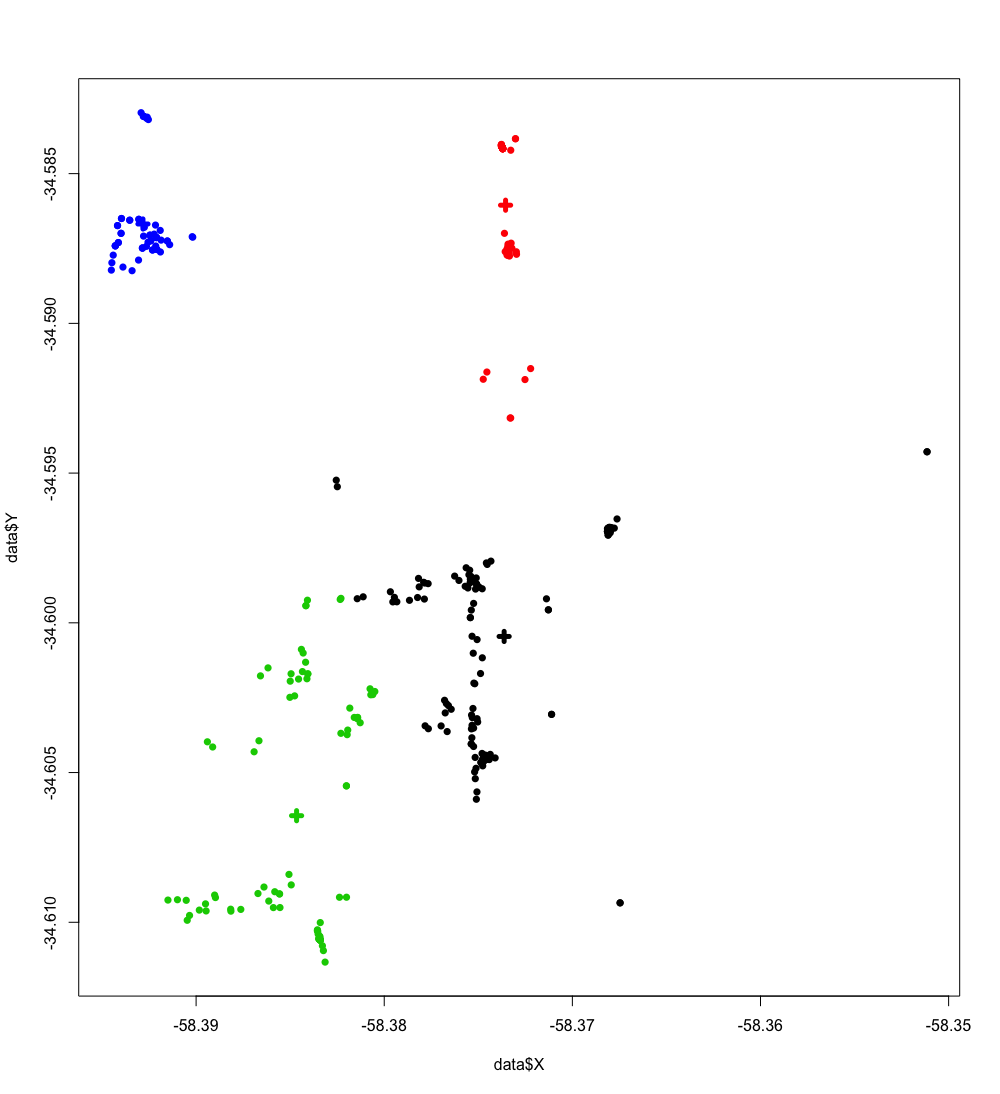
\includegraphics[width=0.8\textwidth]{images/buenosaires-clusters.png} 
				\label{buenosaires-kmeans}
			\end{center}
		\end{figure}
		
		\item To begin the velocity pruning with, the $addVelocityBetweenPoints()$ function calculates the elapsed time between the measured points based on the differences between the timestamps. With the usage of velocity threshold $1 \frac{m}{s}$, the number of points is reduced from 334 to 292. The pruned points and their annotated clusters are displayed on Figure \ref{buenosaires-annottated-clusters}. 
		
		It is visible that the points which formed the previously detected places (clusters) remained in the dataset after the velocity pruning was performed. This further confirms the validity of these places, however some of the clusters on Figure \ref{buenosaires-kmeans} should probably be divided into multiple smaller clusters and yield in more than 4 POIs. 
	
	\begin{figure}[h] 
		\begin{center}
			\caption{The 292 points after the velocity pruning was performed on the Buenos Aires dataset and seven clusters of the dataset which were annotated manually.}
			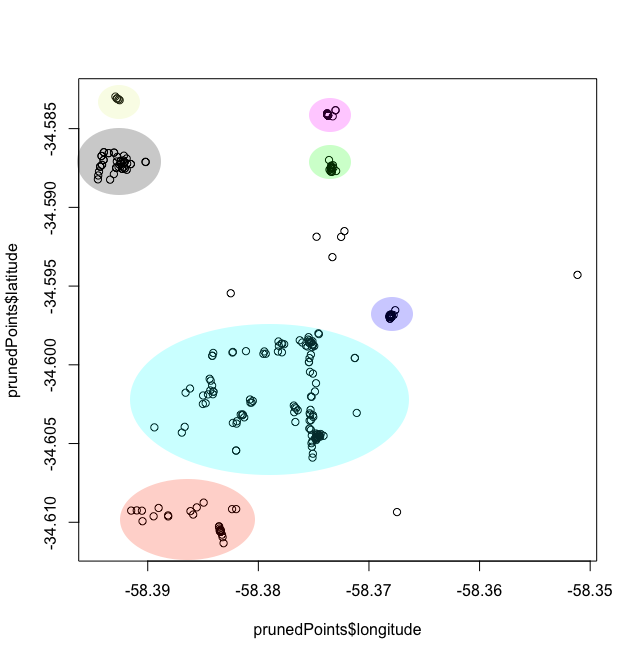
\includegraphics[width=0.8\textwidth]{images/buenosaires-annoted_clusters_after_velocity_pruning.png}
			\label{buenosaires-annottated-clusters}
		\end{center}
	\end{figure}
	
		\item 
	\end{enumerate}
\section{Map Matching}
	\begin{enumerate}[a)]
		\item The attached $map\_matching.R$ file contains the partial solution of this task. Figure \ref{interpolated_points} displays the original points (black) and the new ones added using interpolation technique (red). Using 10 seconds sampling interval, 452 points are added in total. 
		
		\begin{figure}[h] 
		\begin{center}
			\caption{The 193 original measured points (black) in the $cabspotting_trace.csv$ and the 452 new points (red) added using interpolation. }
			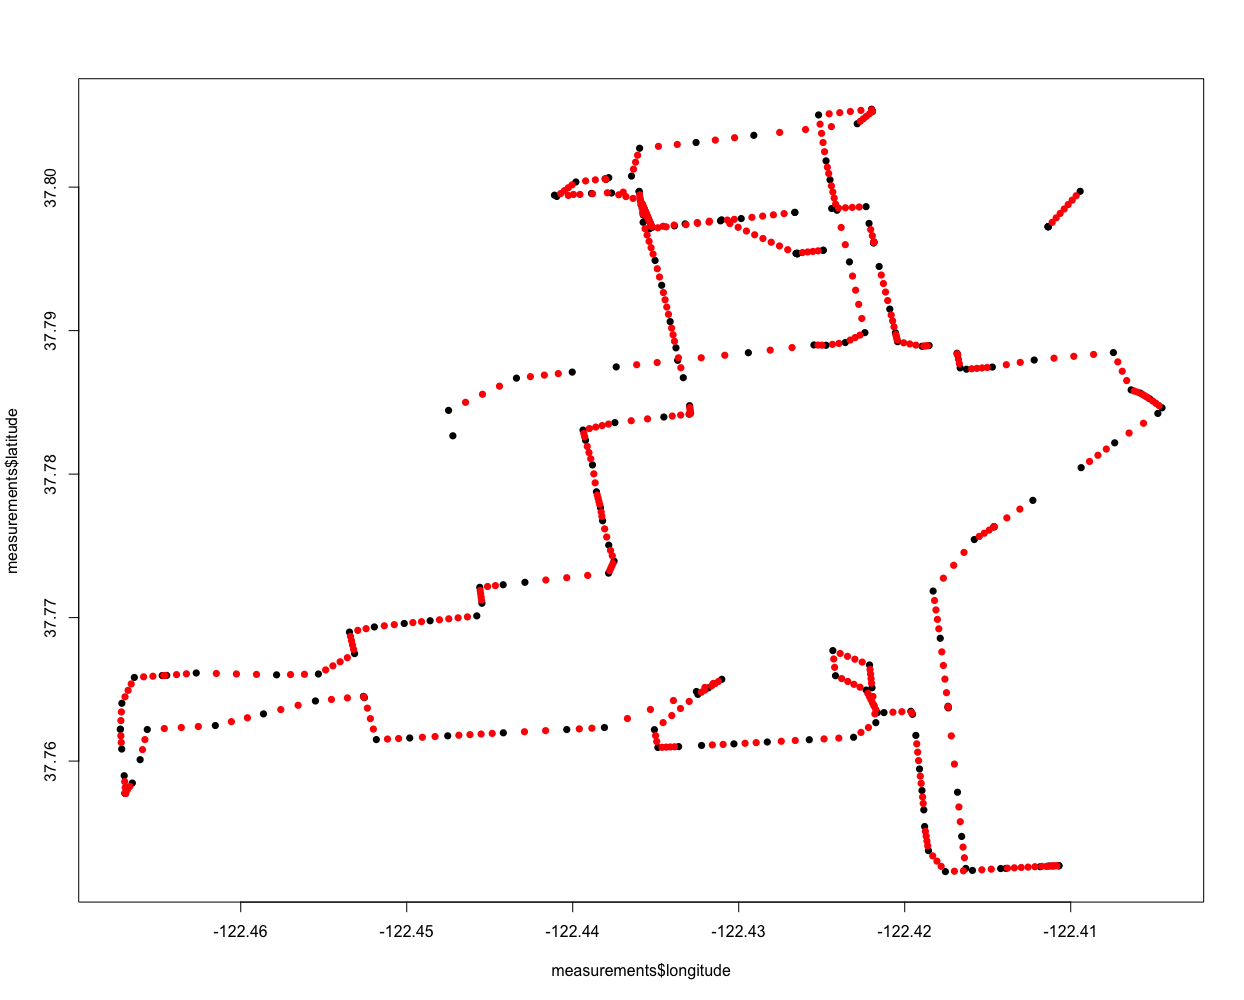
\includegraphics[width=0.8\textwidth]{images/interpolated_points.png}
			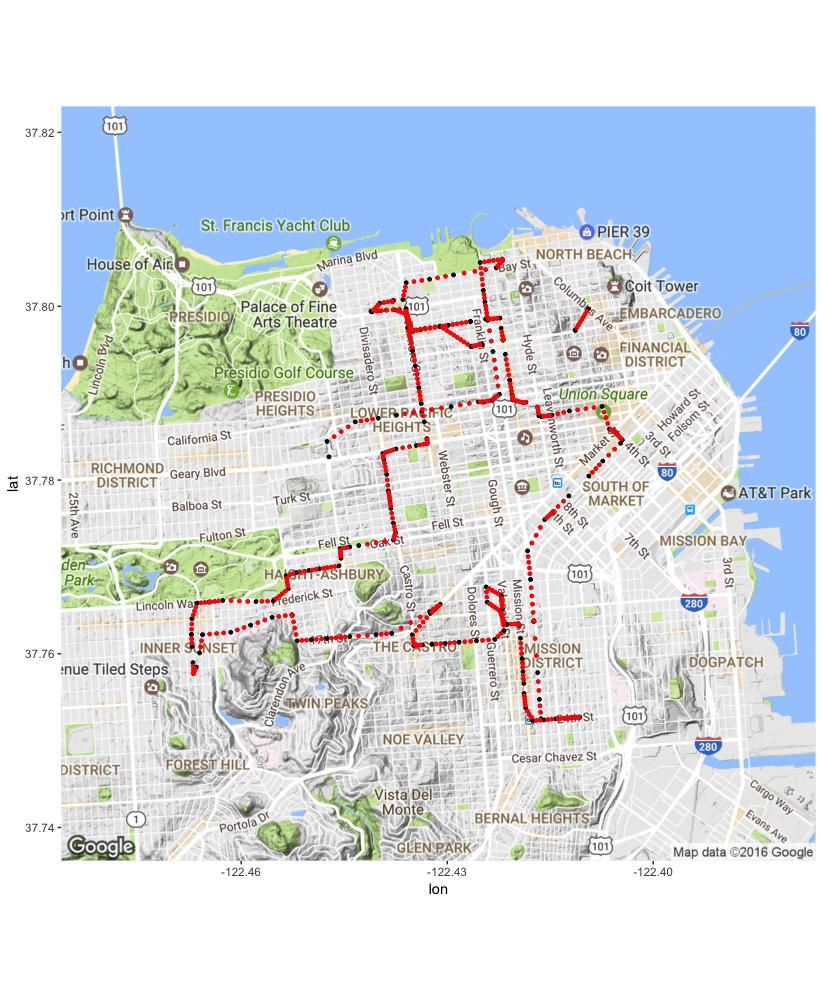
\includegraphics[width=0.8\textwidth]{images/interpolated_points_on_map.png}
			\label{interpolated_points}
		\end{center}
	\end{figure}

	\item The bounding box of the measurements is limited by the two points (-122.4673, 37.80543) (top left point) and (-122.4045, 37.7523) (bottom right item). Unfortunately, the exported OSM file did not load in R and I was unable to perform the analysis. Nevertheless, from the bottom item on Figure \ref{interpolated_points} we can clearly see, that the interpolated points (with red) match in most cases with the road segments, however in some cases they go through buildings as the user was probably taking sequential left and right turns at intersections.
	
	\item 
	\item	
	\end{enumerate}	
	
\nocite{*}
\bibliographystyle{tktl}
\bibliography{lahteet}

\lastpage

\pagestyle{empty}

\end{document}